%
%  長野高専 電子情報工学科 卒業研究発表会 予稿スタイルファイル
%  Version 2019
%
%  作成: 伊藤祥一
%  協力: 大矢健一
%
\documentclass[a4j, 9pt, twocolumn, twoside]{jsarticle}
\usepackage{eipaper}

%  タイトル・著者・指導教員
\newcommand{\Jtitle}{Deep Learningを用いた天気予測}
\newcommand{\JtitleShort}{長野高専 電子情報工学科 卒業研究発表会} % 短縮する場合は\newcommand{\JtitleShort}{わが猫}のようにする
\newcommand{\Etitle}{Weather forecast using Deep Learning}
\newcommand{\Author}{清水 翔仁}  %  姓と名の間に半角スペース
\newcommand{\Teacher}{西村 治}

%  年度と発表月の設定
\newcommand{\Nendo}{2019}  %  年度
\newcommand{\Happyo}{2}    %  2019年度の2月(=2020年2月)に発表会
\setcounter{Nanki}{\number\Nendo}
\addtocounter{Nanki}{-1992}
\setcounter{HappyoYear}{\number\Nendo}
\addtocounter{HappyoYear}{1}

%  ページ番号の設定
\newcommand{\LabSymbol}{H}  % B-5からはじめる
\setcounter{page}{7}


%
%  本文
%
\begin{document}
\twocolumn[\Maketitle]\footnotetext[1]{指導教員: \Teacher}
\section{はじめに}
	現在の情報技術は,第四次産業革命とも呼ばれるほど大きな変化をもたらすと捉えられている.特に「人工知能(AI)」は,火薬と核兵器に次ぐ人類最大の発明とも称され,私達の将来を左右する力を持つと考えられる.また2000年代に「Deep Learning」の手法が開発されて以来,第三次AIブームが起こり,現在も進行中である.

	AI自らが知識を獲得することを「機械学習」という.Deep Learningは,機械学習の一種であるが,ニューラルネットワーク(NN)と呼ばれる人間の脳のメカニズム同様,大量の情報を多層的に処理する手法を用いる点が,従来の機械学習と異なっている.その多層的な情報処理の能力は,注目すべき点である特徴量を人間に支持されなくとも自ら見つけ出すことができる.したがってDeep Learningは,人間が従来認識していなかったような注目点や重要度を提示して「これが知である」という定義を行うことにより,人間の知能を超える可能性を持っている.\cite{rinri}

	Deep Learning技術は画像認識の分野をはじめとして,音声認識,自然言語処理の分野で大きな成果をあげているが,近年では気象予測の分野でもその適用例が報告されている.文献\Cite{kishow}によると,気象庁では三層の順伝播型ネットワークを用いて予測を行っている.これは長いニューラルネットワークの歴史の中で,第二世代に当たる技術である.本研究では,それとは異なる「LSTM」を用いて,翌日の降水の有無を予測する.LSTMとは,テキスト,音声,時系列データなどの入力間に依存性があるデータに対するモデルである.

\section{予備知識}
	本章では,本研究を説明する上で必要な用語について述べる.
	\subsection{モデル}
		モデルとは,コンピュータが分かる形の入力値を受け取り,何かしらの評価・判定をして出力値を出すものである.機械学習やAIにおいて中心的な役割を担う頭脳を意味する.
	\subsection{エポック数}
		エポック数とは,モデルが学習データセットに対して学習した回数である.エポック数が多すぎると「過学習」を起こし,正確な結果が得られない.逆に少なすぎると,モデルの学習が足りないため精度が伸びない.
	\subsection{過学習}
		過学習とは,トレーニングデータセットではうまく機能するモデルが,未知のデータ(テストデータセット)ではうまく汎化されないという問題のことである.その原因は,データに対してモデルが複雑過ぎることや,トレーニングデータセットが足りないことによる学習不足だと考えられる.経験則として,学習中にテストデータの損失が一旦下がったあとに増加したら,それは過学習を起こしている兆候である.\cite{oreilly}
	\subsection{隠れ層}
		隠れ層とは,ニューラルネットワークにおける入力層と出力層以外の層のことである.一般に,隠れ層の数や,一つの層あたりのノード数が多ければ多いほど精度が高くなる.しかし多すぎるとモデルが複雑になってしまい,過学習を引き起こす.
	\subsection{バッチサイズ}
		学習データセットをいくつかに小分けしたかたまりのことをバッチといい,その大きさのことをバッチサイズという.

\section{学習データセット}
	本研究では,気象庁ホームページにて公開されている気象データをダウンロードすることで,学習データセットを作成する.このとき,ダウンロードするデータの条件を指定できる.今回指定した条件を次に示す.
	\begin{itemize}
		\item 期間:1998/1/1 - 2019/12/31
		\item 地点:長野市
		\item 特徴量:日平均現地気圧,日平均気温,日最低気温,日最高気温,降水量の日合計,日照時間,日平均風速,日最大風速,日平均相対湿度,日最小相対湿度,日平均雲量
	\end{itemize}

	また,このままでは特徴量によって値の桁が異なり,分類の精度が低くなってしまうため「正規化」を行う.「正規化」とは値を0〜1の範囲にスケーリングし直すことである.サンプル$x^{\left( i\right) }$の正規化した値$x^{\left( i\right) }_{norm}$を求める式を式(\ref{equ_norm})に示す.
	\begin{equation}\label{equ_norm}
		x^{\left( i\right) }_{norm}=\dfrac {x^{\left( i\right) }-x_{\min }}{x_{\max }-x_{\min }}
	\end{equation}

	式(\ref{equ_norm})において,$x^{\left( i\right) }$は特定のサンプルであり,$x^{\left( i\right) }_{min}$は特徴量の列における最小値,$x^{\left( i\right) }_{\max}$は最大値を表す.\cite{python}

\section{モデルの学習}
	隠れ層が2つの場合と3つの場合についてそれぞれ学習を行った.隠れ層の数以外の条件を以下に示す.

	\begin{itemize}
		\item 隠れ層のノード数:12
		\item バッチサイズ:32
		\item エポック数:128(最大値)
	\end{itemize}

	ここで,エポック数は,過学習の兆候が見られたときにコールバック関数によって学習がストップされるため,最大値のみを定める.また学習の様子はTensorBoard\cite{tb}を用いて観測する.

\section{モデルの評価}
	隠れ層が2つの場合について,テストデータにおける精度の推移を\figref{fig_hidden2_acc},損失の推移を\figref{fig_hidden2_loss}に示す.
	\begin{figure}
		\centering
		\fbox{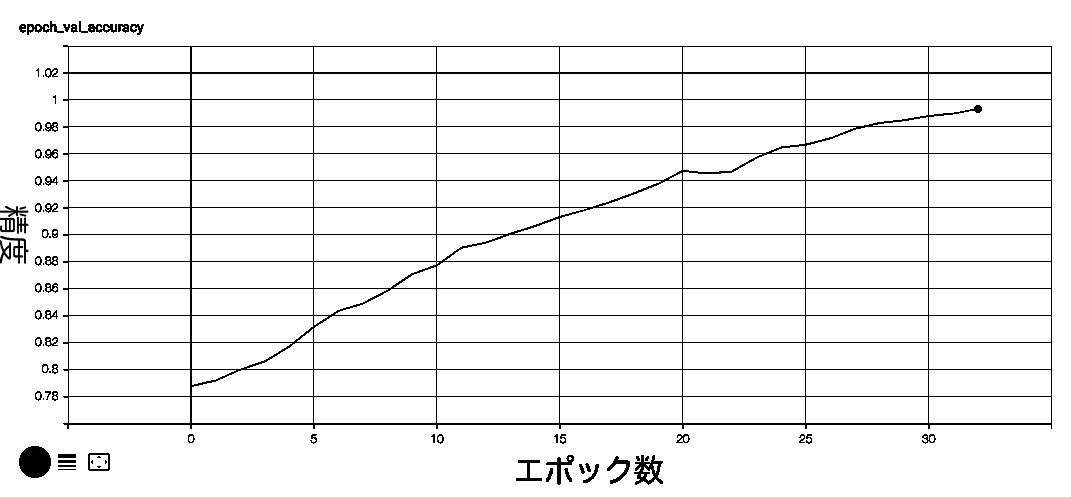
\includegraphics[width=7cm]{./images/hidden2_acc_v3.png}}
		\caption{精度の推移(隠れ層が2つ)}
		\label{fig_hidden2_acc}
	\end{figure}
	\begin{figure}
		\centering
		\fbox{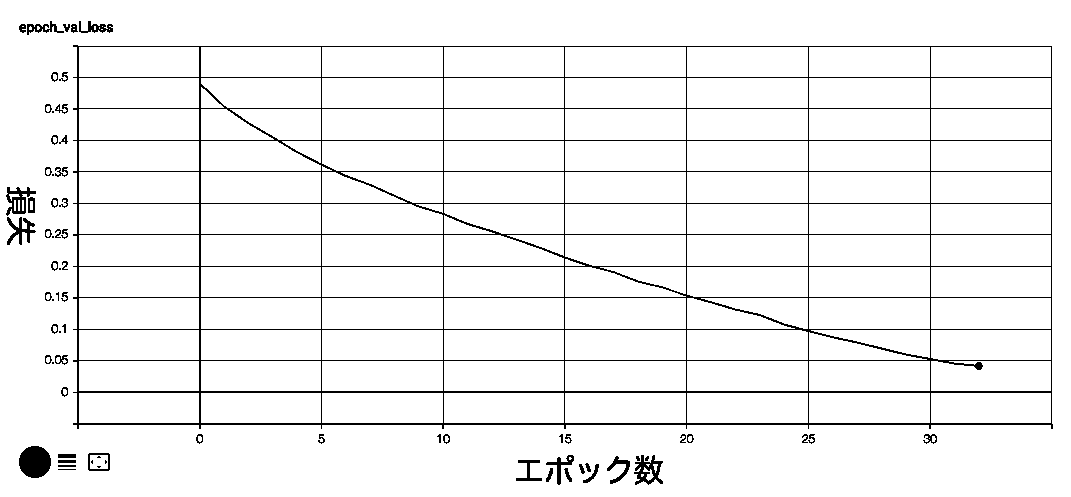
\includegraphics[width=7cm]{./images/hidden2_loss_v3.png}}
		\caption{損失の推移(隠れ層が2つ)}
		\label{fig_hidden2_loss}
	\end{figure}
	\figref{fig_hidden2_acc}より,精度が100\%に近い値になっていることがわかる.また\figref{fig_hidden2_loss}より,エポック数が増えるたびに順調に損失が下がっていることがわかる.

	隠れ層が3つの場合について,テストデータにおける精度の推移を\figref{fig_hidden3_acc},損失の推移を\figref{fig_hidden3_loss}に示す.
	\begin{figure}
		\centering
		\fbox{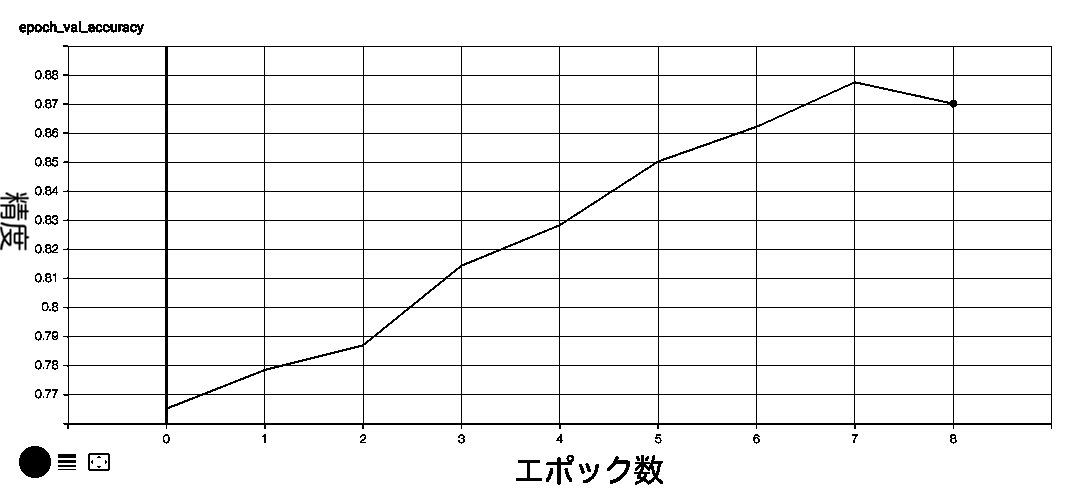
\includegraphics[width=7cm]{./images/hidden3_acc_v3.png}}
		\caption{精度の推移(隠れ層が3つ)}
		\label{fig_hidden3_acc}
	\end{figure}
	\begin{figure}
		\centering
		\fbox{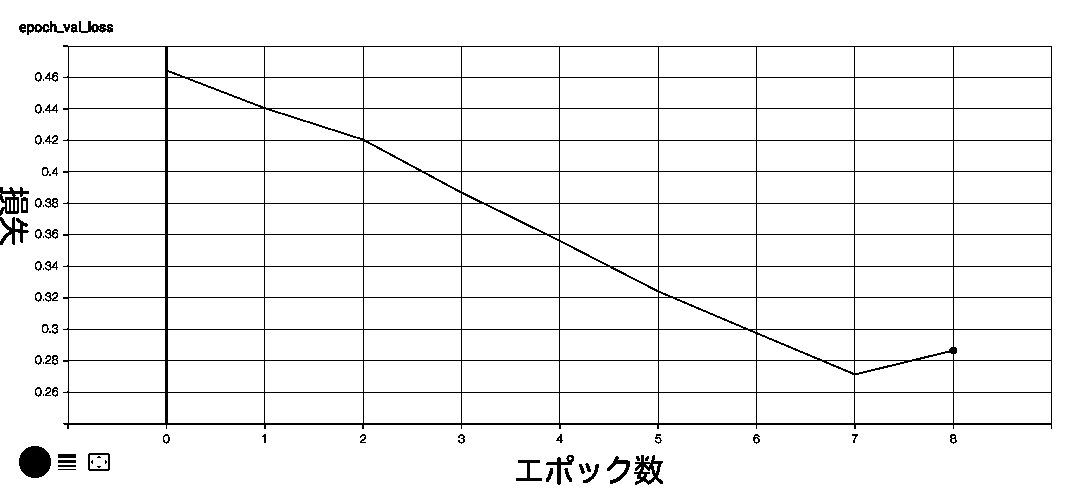
\includegraphics[width=7cm]{./images/hidden3_loss_v3.png}}
		\caption{損失の推移(隠れ層が3つ)}
		\label{fig_hidden3_loss}
	\end{figure}
	\figref{fig_hidden3_acc}より,エポック数が7の時点で精度が頭打ちになり,エポック数8で学習が終了していることがわかる.また\figref{fig_hidden3_loss}より,下がり続けた損失がエポック数7から上昇しており,過学習が起きていることがわかる.

	これらの結果から,隠れ層の数は2が妥当であると考えられる.

\section{まとめ}
	Deep Learningを用いて,気象観測データから翌日の降水の有無を予測することができた.この方法を用いれば長野市に限らず,その他の地域でも予測が可能であると考えられる.
	課題として,現在は日別の降水のみを予測しているため,何時に雨が降るかという予測はできない.これは,学習データセットを1時間毎の観測データに変更することで,1時間毎の降水を予測できると考えられる.また,今回は気象庁ホームページからダウンロードしたデータを手作業で整形している.この作業を全てプログラム内で行うことによって,研究をより効率化できると考えられる.

\begin{thebibliography}{9}
\bibitem{rinri}{鬼頭 葉子: 技術者の倫理, ナカニシヤ出版, 2018.}
\bibitem{kishow}{気象庁 | 数値予報課報告・別冊第64号(令和2年1月20日現在): \url{https://www.jma.go.jp/jma/kishou/books/nwpreport/64/chapter5.pdf}}
\bibitem{oreilly}{Antonio Gulli・Sujit Pal(著),大串正矢・久保隆宏・中山光樹(訳): 直感Deep Learning, 株式会社オライリー・ジャパン, 2019.}
\bibitem{python}{Sebastian Raschka・Vahid Mirjalili(著),株式会社クイープ(訳): [第2版]Python機械学習プログラミング, 株式会社インプレス, 2018.}
\bibitem{tb}{TensorBoard(令和2年1月20日現在): \url{https://www.tensorflow.org/tensorboard}}
\end{thebibliography}

\end{document}
